\documentclass[logo,reportComp]{thesis}
\usepackage[cpp,pseudo]{mypackage}

\title{分布式系统作业四}
\subtitle{}
\school{数据科学与计算机学院}
\author{陈鸿峥}
\classname{17大数据与人工智能}
\stunum{17341015}
\headercontext{分布式系统作业}

\begin{document}

\maketitle

\begin{question}
在深度为$k$的分层定位服务中,当移动实体改变它的位置时,最多需要更新多少条位置记录?
\end{question}
\begin{answer}
假设该实体移动到根节点的另一分支中。
先做删除操作,指针链上的结点记录都会被修改,一共$k+1$个;
其次做插入操作,同样新分支上指针链的所有结点记录都会被修改,一共$k+1$个。
但由于根结点被重复计算,所以一共
\[(k+1)+(k+1)-1=2k+1\]
条记录需要被更新。
\end{answer}

\begin{question}
分层定位服务中的根节点可能是一个潜在的瓶颈。如何能有效地避免这个问题?
\end{question}
\begin{answer}
可以采用分布式的方案。
将根节点的记录进行划分,然后分别存储在不同的机器上。
当根节点的孩子需要通过根结点查找记录时,先对查找的范围进行定位,然后再到对应的机器上查找记录。
\end{answer}

\begin{question}
请解释如何使用DNS来实现基于宿主位置的方法以定位移动主机。
% Explain how DNS can be used to implement a home-based approach to locating mobile hosts.
\end{question}
\begin{answer}
每一次DNS名字被解析时,都会返回主机当前的IP地址。
而每一次主机移动时,都需要告知其名字服务器新的IP地址。
进而可以通过这种方式来定位移动主机,但注意需要确保名字服务器并未采用cache机制。
\end{answer}

\begin{question}
设置自己的DNS服务器。
在Windows或者Linux操作系统上,安装BIND软件,并为一些简单的名称配置它。
使用诸如Domain Information Groper (DIG)的软件来测试你的配置。
应确保你的DNS数据库包含有名称服务器、邮件服务器和标准服务器的记录。
注意,如果你是在名为\verb'HOSTNAME'的机器上运行BIND,就能解析形如\verb'RESOURCE-NAME.HOSTNAME'的名称。
\end{question}
\begin{answer}
参考\cite{bib1}和\cite{bib2},在Linux环境下安装了bind9,并配置主机名为\verb'chhzh.local',配置好DNS数据库后用dig对域名进行查询。
前向解析结果如下
\begin{figure}[H]
\centering
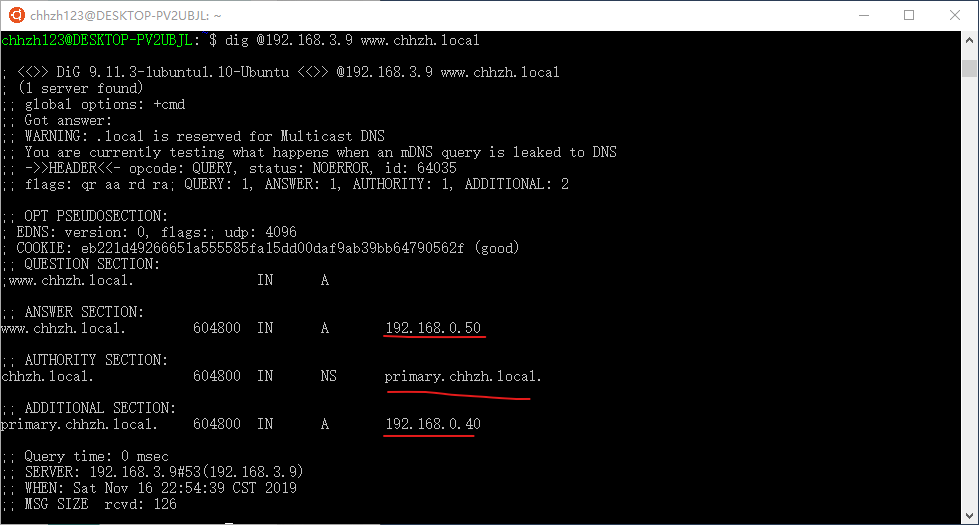
\includegraphics[width=\linewidth]{fig/forward.png}
\end{figure}
反向解析结果如下
\begin{figure}[H]
\centering
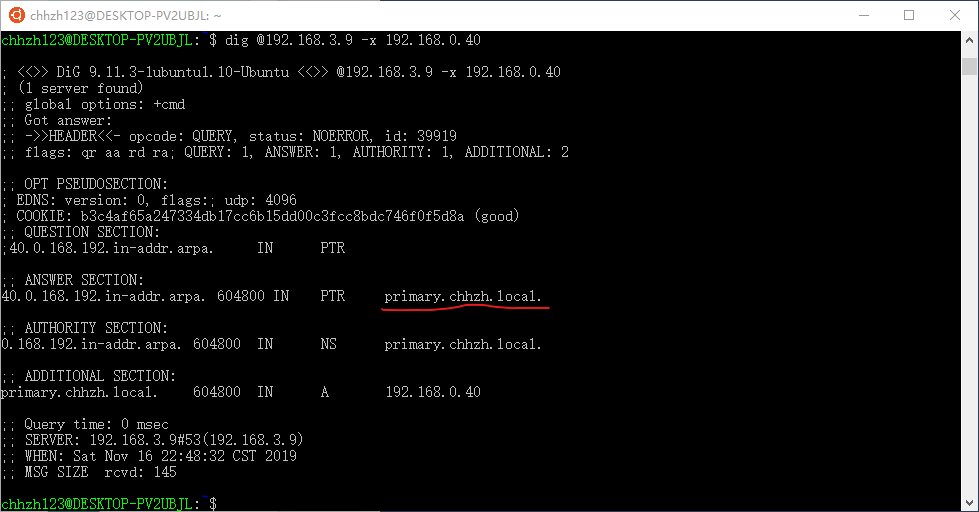
\includegraphics[width=\linewidth]{fig/reverse.png}
\end{figure}
可以看见DNS服务器正常运行。
\end{answer}

\begin{thebibliography}{99}
\bibitem{bib1} Linux DNS server BIND configuration, \url{https://linuxconfig.org/linux-dns-server-bind-configuration}
\bibitem{bib2} How to Install and Configure Bind 9 (DNS Server) on Ubuntu / Debian System, \url{https://www.linuxtechi.com/install-configure-bind-9-dns-server-ubuntu-debian/}
\end{thebibliography}

\end{document}